\documentclass[aspectratio=169]{beamer}
\usepackage[utf8]{inputenc}
\usepackage[T1]{fontenc}
\usepackage[brazilian]{babel}
%\useoutertheme{infolines} %tema externo
%\useinnertheme{rectangles} %tema interno
%\beamertemplatenavigationsymbolsempty %retirar a barra de navegação
\usepackage{graphicx} %IMAGEM
\usepackage{multicol, indentfirst}
\usepackage{amsmath, amssymb, amsthm}  %Matemática
\usepackage{lipsum} %texto de preenchimento em latim
\usepackage{xcolor}

\usepackage[alf]{abntex2cite}



% pasta das imagens
\graphicspath{ {./img/} }

% comando para compilar com ou sem pausas (condição: comentário abaixo)
\newcommand{ \conditionalcomment }[1]{
	%#1 	% comente essa linha para que esses comandos não sejam compilados 
}	% exemplo de uso: \conditionalcomment{\pause}



% comando para formatar o nome de todos os solvers igual
\newcommand{ \solver }[1]{\textit{#1}}	



%Redefinindo as cores da SEMAT
\definecolor{laranja}{RGB}{0, 68, 0}
\definecolor{azul}{RGB}{0,0,0}%{1, 146, 63}
\definecolor{verde}{RGB}{21, 76, 0}

%Cores das estruturas do beamer
\setbeamercolor{author}{fg=azul}
\setbeamercolor{title}{fg=laranja}
\setbeamerfont{title}{size=\LARGE, series=\bf}

\setbeamercolor{}{fg=laranja}
\setbeamercolor{frametitle}{fg=laranja}
\setbeamerfont{frametitle}{series=\bf}

\setbeamercolor{structure}{fg=laranja}
\setbeamercolor{block body alerted}{}
\setbeamercolor{block title alerted}{fg=black, bg=azul!50}
\setbeamercolor{block body example}{fg=black}
\setbeamercolor{block title example}{fg=verde}
\setbeamercolor{block title}{fg=verde}
\setbeamercolor{block body}{bg=laranja!10, fg=black}

%cabeçalho
\setbeamertemplate{headline}{}

%rodapé
\setbeamertemplate{footline}{}

\date{\href{https://www.uel.br/}{\includegraphics[height=0.15\textheight]{Logo_UEL.png}} \quad
	\href{https://www.uel.br/eventos/verao/2023/painel-alunos.html}{\includegraphics[height=0.16\textheight]{LOGO.png}} \quad
	\href{https://www.uel.br/pos/pgmac}{\includegraphics[height=0.16\textheight]{Logo_pgmac.png}}}
%----------------------------%
%personalize daqui para baixo:



%informações do autor:
\title{Avaliação de resolvedores para problemas de localização de facilidades com capacidade limitada}

\author{Guilherme Akira Demenech Mori
	\qquad \qquad Aline A. S. Leão
	\\	\texttt{akira.demenech@uel.br}
	\qquad \qquad \qquad 
	\texttt{aasleao@uel.br}}

\institute{\href{https://picme.obmep.org.br/}{\includegraphics[height=0.13\textheight]{Logo_picme.png}}}

\begin{document}



	\begin{frame} % título inicial
		\maketitle
	\end{frame}

	
	\begin{frame}{Problemas de localização de facilidades com capacidade limitada (CFLP)}
		% 								 			
		No CFLP são minimizados os custos de instalação de facilidades e de designação de clientes a elas, de forma a respeitar as limitações de capacidade das facilidades e a satisfazer as demandas dos clientes. 

		\begin{figure}[H]
			\begin{center}
				\caption{Clusterizações de conjuntos de dados aleatórios}
				
				\includegraphics[width=0.3\textwidth]{clustering birch.png}
				\hfill 
				\includegraphics[width=0.3\textwidth]{clustering birch s65432 c3.png}
				\hfill 
				\includegraphics[width=0.3\textwidth]{clustering birch s957 c5.png}
				\label{ilustr:birch}
				
				\textbf{Fonte}: autoria própria.
			\end{center}
		\end{figure}
			
			
		
	\end{frame}	

	\begin{frame}{Literatura}
		
		\begin{itemize}
			\item \textbf{Localização de facilidades}: 
				começo do século XX				
				\\ Alfred Weber 
				
			\item \textbf{Problema de localização simples (SPLP)}: 
				década de 1960	
				\\ Michel Balinski e outros 
		\end{itemize}	
		\cite{Labbe,Krarup}.	 

		%\vfill

	\end{frame}	

	\begin{frame}{Aplicações}
	
		%\framesubtitle{Aplicações}
		\begin{multicols}{2}
			\begin{itemize}
				\item Armazéns
				\item Fábricas
				\item Centros de distribuição
				\item Hospitais
				\item Escolas
				\item Componentes eletrônicos
				\item Fornecedores 
			\end{itemize}	
		\end{multicols}
		
		\cite{Arenales,Krarup,Klose}

		\begin{figure}[H]
			\begin{center}
				\caption{Representação do problema como um grafo bipartido}
				
				\includegraphics[width=0.5\textwidth]{grafo bipartido.png}				
				\label{ilustr:bigrafo}
				
				\textbf{Fonte}: autoria própria.
			\end{center}
		\end{figure}
		
		
	\end{frame}


	\begin{frame}{Problema de localização de facilidades com capacidade limitada com múltiplas fontes (MS-CFLP)}
		% Definição e Variantes	
		\framesubtitle{Cada demanda pode ser suprida por mais do que uma facilidade}
		
		 
		
		
		
		
		%minimize
		\begin{equation}
			\label{ms:obj}		
			\min \sum_{i \in I} 
			(
			f_i y_i + \sum_{j \in J} c_{ij} x_{ij}
			)
		\end{equation}
		
		sujeito a 				
		
		\begin{equation}
			\label{ms:const:demand}		
			\sum_{i \in I} x_{ij} \ge d_j 
			\quad
			\forall j \in J
		\end{equation}
	
		\begin{equation}
			\label{ms:const:capacity}		
			\sum_{j \in J} x_{ij} \le y_i s_i 
			\quad
			\forall i \in I
		\end{equation}

		\begin{equation}
			\label{ms:dom:var}		
			y_i \in \{0, 1\}, 
			\ x_{ij} \ge 0, 
			\ x_{ij} \in \mathbb{Z}
			\quad
			\forall i \in I, \ j \in J
		\end{equation}
		
	\end{frame}	

	\begin{frame}{Problema de localização de facilidades com capacidade limitada com fonte única (SS-CFLP)}
		% Definição e Variantes	
		\framesubtitle{Cada cliente deve ser atendido inteiramente por só uma facilidade}

		\begin{equation}
			\label{ss:obj}		
			\min \sum_{i \in I} 
			(
			f_i y_i + \sum_{j \in J} c_{ij} x_{ij}
			)
		\end{equation}
		
		sujeito a 				
		
		\begin{equation}
			\label{ss:const:demand}		
			\sum_{i \in I} x_{ij} \ge d_j 
			\quad
			\forall j \in J
		\end{equation}
	
		\begin{equation}
			\label{ss:const:capacity}		
			\sum_{j \in J} x_{ij} \le y_i s_i 
			\quad
			\forall i \in I
		\end{equation}
	
		\begin{equation}
			\label{ss:const:int}		
			\boldsymbol{x_{ij} = d_j z_{ij}}  
			\quad
			\boldsymbol{\forall i \in I, \ j \in J}
		\end{equation}

		\begin{equation}
			\label{ss:dom:var}		
			\boldsymbol{z_{ij} \in \{0,1\}},
			y_i \in \{0, 1\}, 
			\ x_{ij} \ge 0, 
			\ x_{ij} \in \mathbb{Z}
			\quad
			\forall i \in I, \ j \in J
		\end{equation}
		
		
		
		
		
	\end{frame}

	\begin{frame}{Problema de localização de facilidades com capacidade limitada com incompatibilidade de clientes (MS-CFLP-CI)}
		% Definição e Variantes	
		\framesubtitle{Alguns clientes não podem ser atendidos pela mesma facilidade}
		
		\begin{equation}
			\label{ci:obj}		
			\min \sum_{i \in I} 
			(
			f_i y_i + \sum_{j \in J} c_{ij} x_{ij}
			)
		\end{equation}
		
		sujeito a 				
		
		\begin{equation}
			\label{ci:const:demand}		
			\sum_{i \in I} x_{ij} \ge d_j 
			\quad
			\forall j \in J
		\end{equation}
	
		\begin{equation}
			\label{ci:const:capacity}		
			\sum_{j \in J} x_{ij} \le y_i s_i 
			\quad
			\forall i \in I
		\end{equation}

		\begin{equation}
			\begin{aligned}
				\label{ci:const:incomp}		
				& \boldsymbol{x_{ij_1} \le \lambda_{ij_1j_2} s_i}, 
				\\ & \boldsymbol{x_{ij_2} \le (1 - \lambda_{ij_1j_2}) s_i} 
				\quad
				\boldsymbol{\forall i \in I}, 
				\ \boldsymbol{\{ j_1, j_2 \} \in \Gamma}  
			\end{aligned}
		\end{equation}
	
		

		\begin{equation}
			\label{ci:dom:var}		
			y_i \in \{0, 1\}, 
			\ x_{ij} \ge 0, 
			\ x_{ij} \in \mathbb{Z},				
			\ \boldsymbol{\lambda_{ij_1j_2} \in \{ 0, 1 \}}	
			\quad
			\forall i \in I, \ j \in J,			
			\ \boldsymbol{\{ j_1, j_2 \} \in \Gamma}	
		\end{equation}
		
		
		
		  
		
		
		
		
		
	\end{frame}

	\begin{frame}{Objetivo}

		\begin{block}{}
			Comparar o desempenho dos resolvedores para instâncias do CFLP.	  
		\end{block}
		
		Guiar na escolha de resolvedores levando em consideração os seus recursos disponíveis e o investimento financeiro.
		
		%Coletar dados de quantidade de nós visitados e cortes aplicados para testes com diferentes limites de tempo.

		
		
	\end{frame}

	
	\begin{frame}{Testes}
		% Python, Solvers, Computadores
		
		Modelagem em Python, 
		executando os resolvedores 
		\solver{Gurobi Optimizer}, 
		\solver{IBM ILOG CPLEX} e 
		\solver{COIN-OR Branch-and-Cut} (\solver{Cbc})
		com chamadas da biblioteca PuLP.
		
		\hfill
		
		Parâmetros dos resolvedores foram mantidos na configuração padrão.
		
		\hfill
		
		Os resolvedores comerciais \solver{Gurobi} e \solver{CPLEX} utilizaram até 12 threads.
		
		O resolvedor de código-aberto \solver{Cbc} utilizou apenas 1 thread.
		
		\hfill
		
		Foram analisados resultados com base no tempo limite imposto, os nós de árvore visitados e o gap de otimalidade.
		
		
		\qquad \hfill 
			gap = $100\% \dfrac{\hat{z} - z_{LI}}{z_{LI}}$ 
		\hfill \qquad 
	
	\end{frame}
	
	
	\begin{frame}{Testes}			
		
		\begin{exampleblock}{Instâncias}
			\begin{itemize}
				\item \textbf{Categoria 1}: 
					SS-CFLP \cite{Sobolev}$^1$
					\\ 100 médias: 100 facilidades e 100 clientes
					
					
				\item \textbf{Categoria 2}: 
					SS e MS \cite{Beasley}$^2$
					\\ 24 pequenas: até 50 facilidades e 50 clientes   
					\\ 12 grandes: 100 facilidades e 1000 clientes  
	
				\item \textbf{Categoria 3}:  
					MS-CFLP-CI \cite{Maia}$^3$
					\\ 20 muito grandes: de 50 até 3000 facilidades e de 115 até 7800 clientes 
					\\ 1 muito pequena: 4 facilidades e 10 clientes
			\end{itemize}
		
			
		\end{exampleblock}

		$^1$ Disponível em: \href{http://old.math.nsc.ru/AP/benchmarks/CFLP/cflp_tabl-eng.html}{\textit{math.nsc.ru/AP/benchmarks/CFLP/cflp\_tabl-eng.html}}

		$^2$ Disponível em: \href{http://groups.di.unipi.it/optimize/Data/MEX.html}{\textit{groups.di.unipi.it/optimize/Data/MEX.html}}

		$^3$ Disponível em: \href{https://www.ants-lab.it/mess2020/\#competition}{\textit{ants-lab.it/mess2020}}
		
	\end{frame}


	\begin{frame}{Testes: categorias 1 e 2}
		% Python, Solvers, Computadores
		
		Limite de tempo de 2, 5 e 10 minutos
		\\ \hfill \\
		Computador desktop Ubuntu (i7 64-bit RAM 16 GB)				
		\\ 6 núcleos físicos, 12 processadores lógicos
		
		%Utilizados os limites de tempo de 2, 5 e 10 minutos para todas as instâncias pequenas, médias e grandes dos MS e SS-CFLP \cite{Beasley,Sobolev} num c.
			
		%Para as instâncias do MS-CFLP-CI \cite{Maia} foram utilizados 10, 30 e 60 minutos num laptop Windows 10 (i7 64-bit RAM 16 GB).
	\end{frame}


	\begin{frame}{Resultados: categoria 1 (fonte única)} % Sobolev SS Opt/T
		%\framesubtitle{}
	
		\begin{figure}[H]
			\begin{center}
				\caption{Instâncias médias resolvidas com otimalidade pelo tempo limite SS-CFLP \cite{Sobolev}}
				
				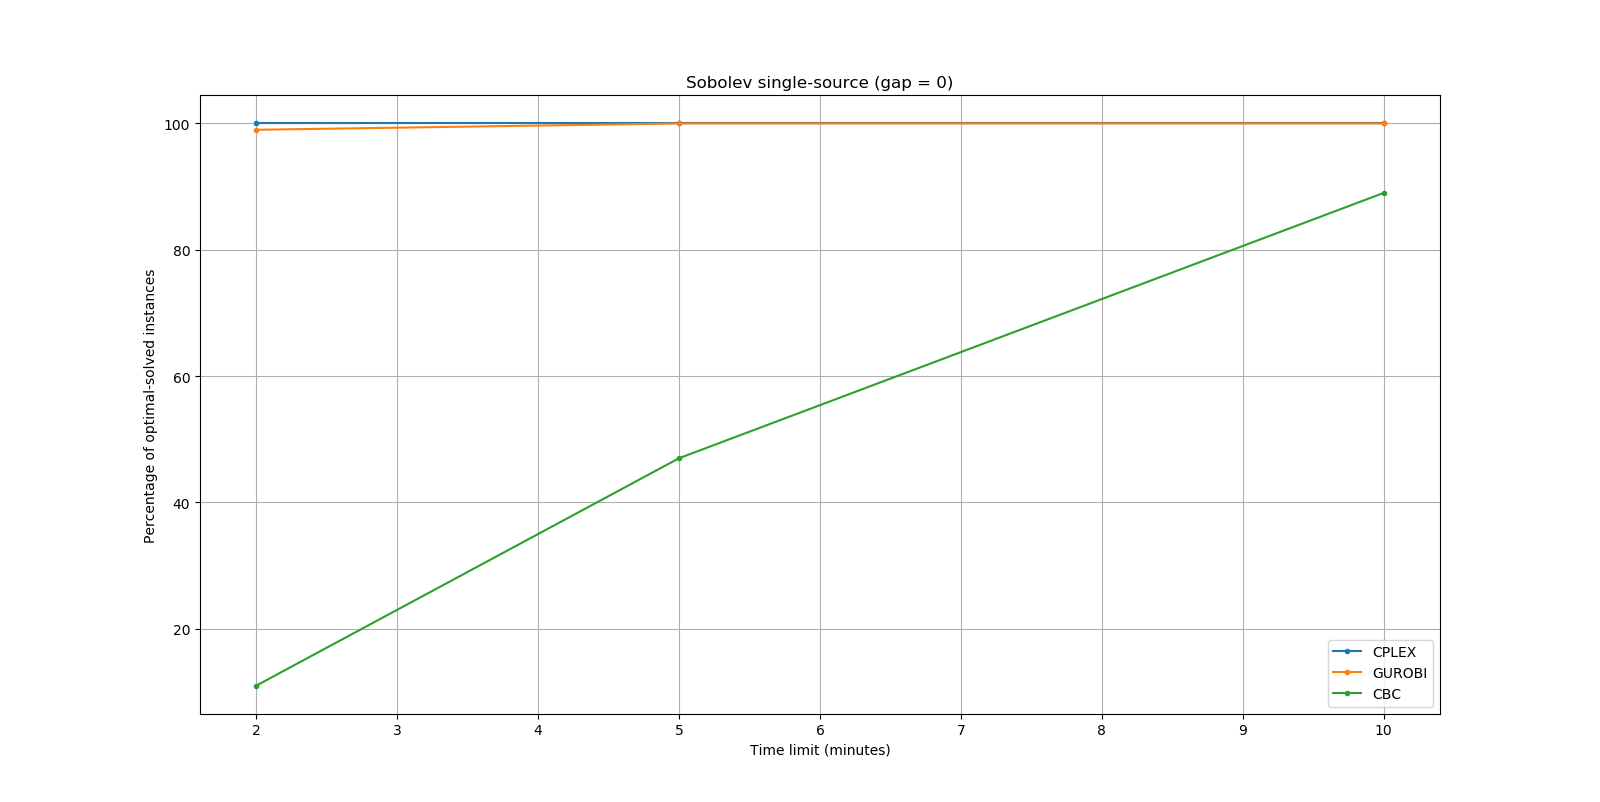
\includegraphics[height=0.6\textheight]{res/Sobolev SS - Optimal x Time.png}
				\label{Opt:T:SS:Sobolev}
				
				\textbf{Fonte}: autoria própria.
			\end{center}
		\end{figure}
	
	\end{frame}

	\begin{frame}{Resultados: categoria 2 (fonte única)} % Beasley SS Opt/T
		%\framesubtitle{}
		
		\begin{figure}[H]
			\begin{center}
				\caption{Instâncias pequenas e grandes resolvidas com otimalidade pelo tempo limite SS-CFLP \cite{Beasley}}
				
				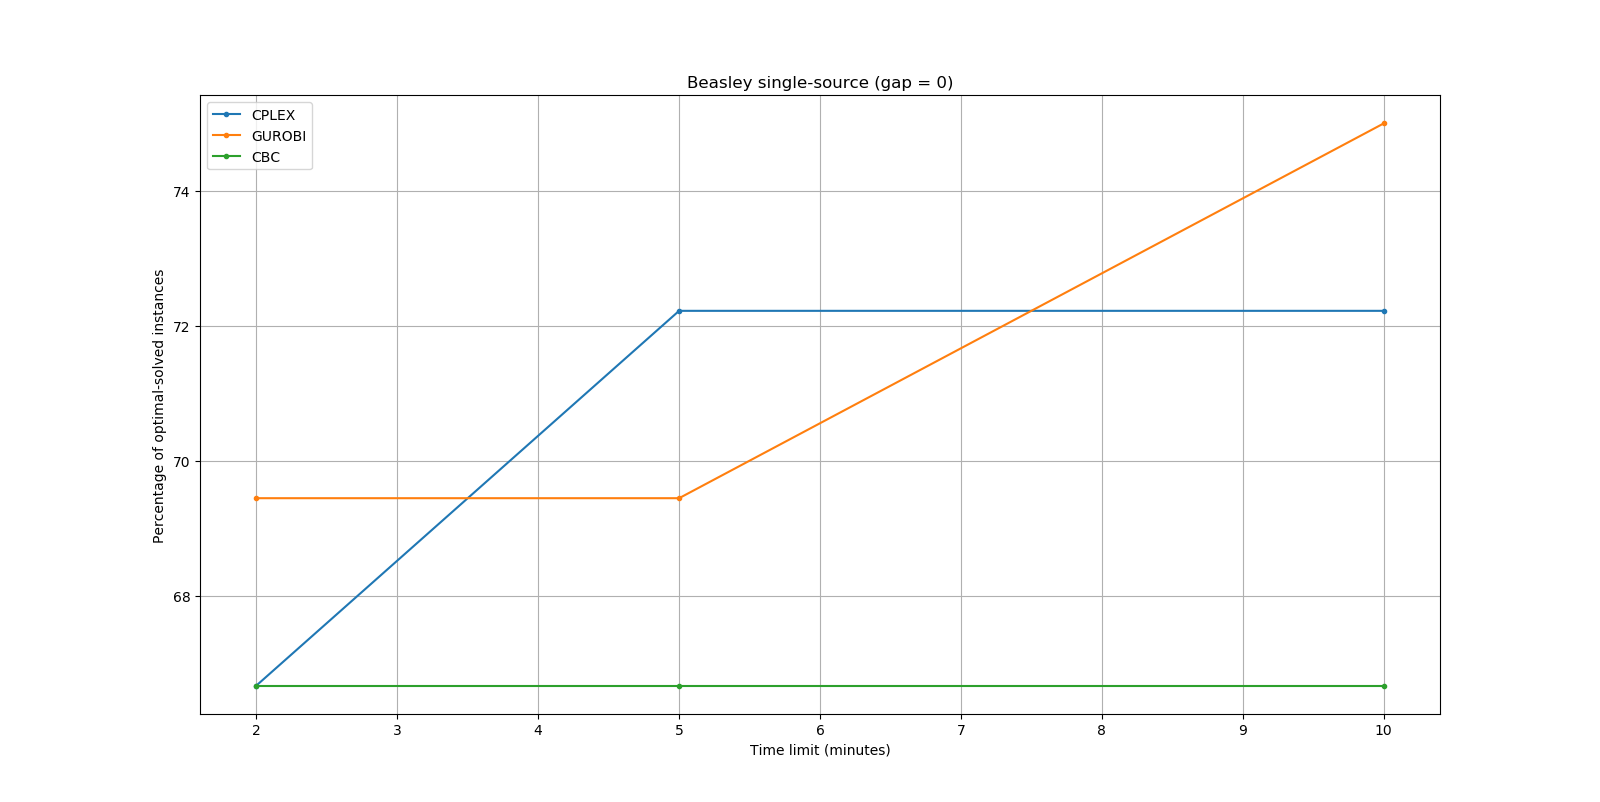
\includegraphics[height=0.6\textheight]{res/Beasley SS - Optimal x Time.png}
				\label{Opt:T:SS:Beasley}
				
				\textbf{Fonte}: autoria própria.
			\end{center}
		\end{figure}
		
	\end{frame}

	\begin{frame}{Resultados: categoria 2 (múltiplas fontes)} % Beasley MS Opt/T
		%\framesubtitle{}
		
		\begin{figure}[H]
			\begin{center}
				\caption{Instâncias pequenas e grandes resolvidas com otimalidade pelo tempo limite MS-CFLP \cite{Beasley}}
				
				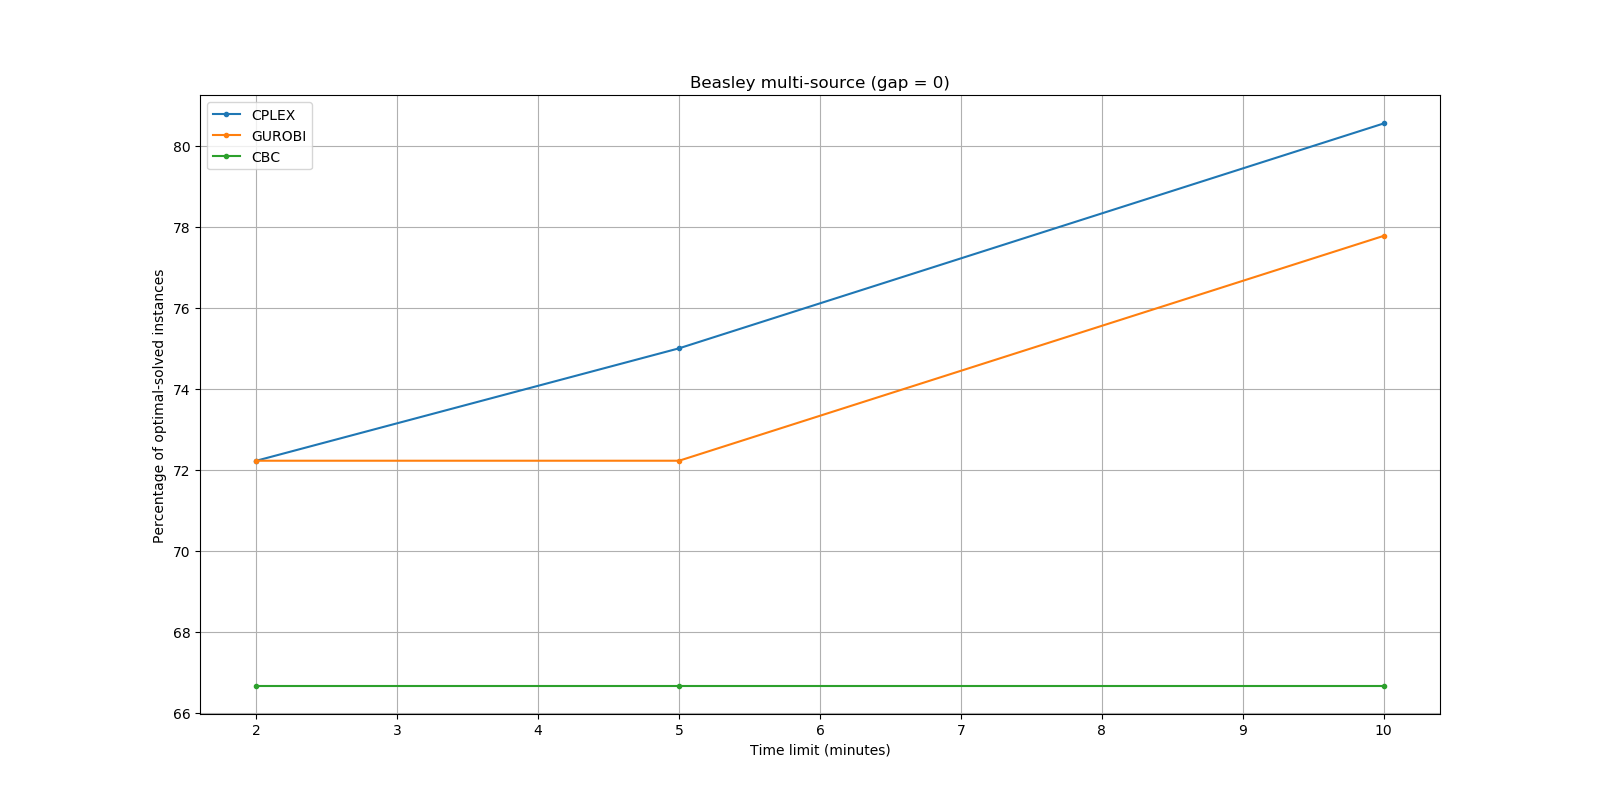
\includegraphics[height=0.6\textheight]{res/Beasley MS - Optimal x Time.png}
				\label{Opt:T:MS:Beasley}
				
				\textbf{Fonte}: autoria própria.
			\end{center}
		\end{figure}
		
	\end{frame}
	
	
	
	
	\begin{frame}{Resultados: categoria 2 (Grandes)} % Beasley Gap/T
		%\framesubtitle{}
		
		\begin{figure}[H]
			\begin{center}
				\caption{Gap médio por tempo limite das instâncias grandes \cite{Beasley}}
				
				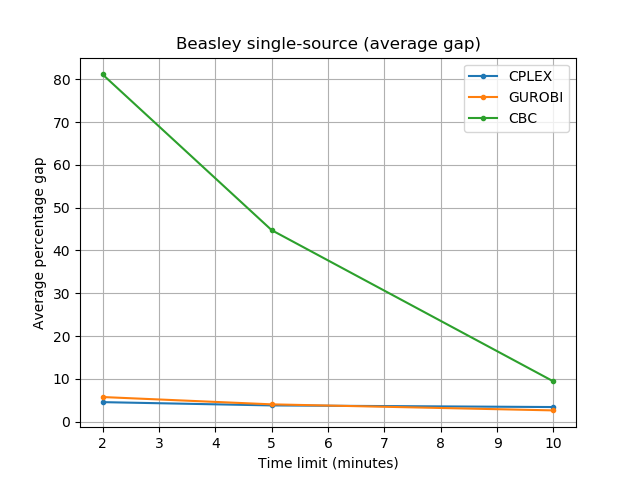
\includegraphics[width=0.49\textwidth]{res/Beasley SS large - Average gap x Time.png}
				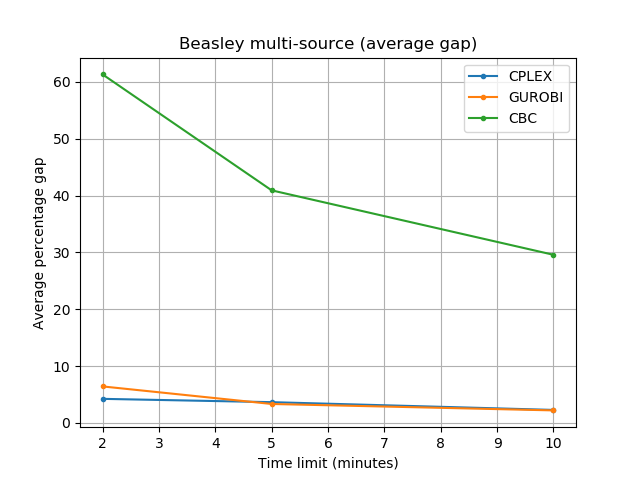
\includegraphics[width=0.49\textwidth]{res/Beasley MS large - Average gap x Time.png}
				\label{Gap:T:Beasley}
				
				\textbf{Fonte}: autoria própria.
			\end{center}
		\end{figure}
		
	\end{frame}
	
	\begin{frame}{Resultados: categoria 2 (Grandes: 2 minutos)} % Beasley 120 Gap/n 
		%\framesubtitle{}
		
		\begin{figure}[H]
			\begin{center}
				\caption{Gap médio das instâncias grandes resolvidas em até $x$ nós e 2 minutos \cite{Beasley}}
				
				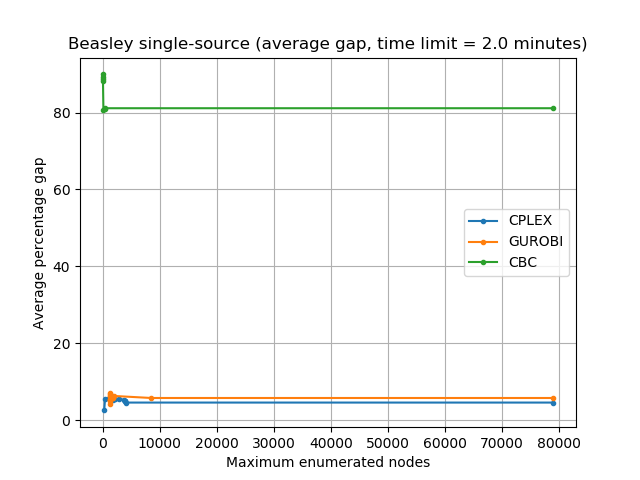
\includegraphics[width=0.49\textwidth]{res/Beasley SS large 120 - Average gap x Nodes.png}
				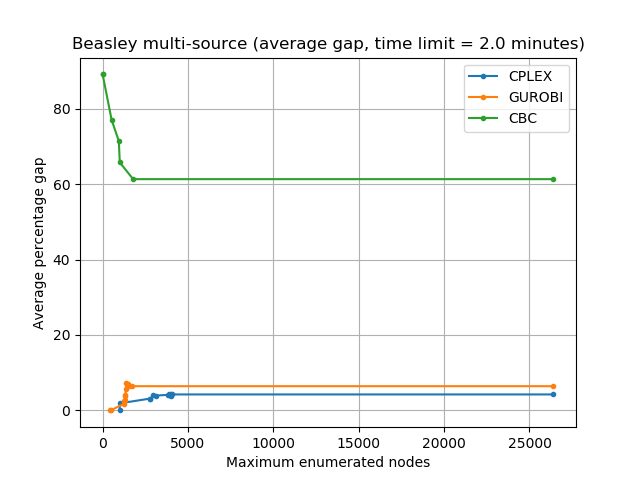
\includegraphics[width=0.49\textwidth]{res/Beasley MS large 120 - Average gap x Nodes.png}				
				\label{Gap:n:Beasley:120}
				
				\textbf{Fonte}: autoria própria.
			\end{center}
		\end{figure}
		
	\end{frame}

	\begin{frame}{Resultados: categoria 2 (Grandes: 5 minutos)} % Beasley 300 Gap/n 
		%\framesubtitle{}
		
		\begin{figure}[H]
			\begin{center}
				\caption{Gap médio das instâncias grandes resolvidas em até $x$ nós e 5 minutos \cite{Beasley}}
				
				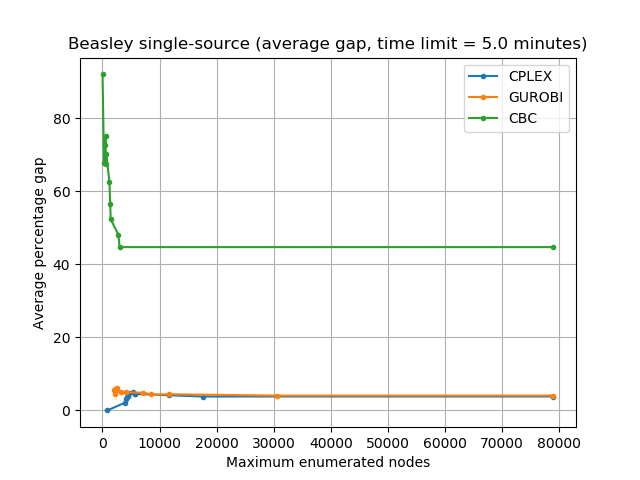
\includegraphics[width=0.49\textwidth]{res/Beasley SS large 300 - Average gap x Nodes.png}
				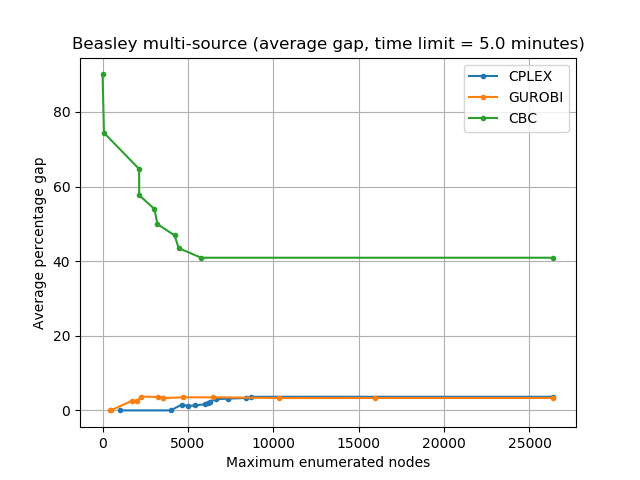
\includegraphics[width=0.49\textwidth]{res/Beasley MS large 300 - Average gap x Nodes.png}				
				\label{Gap:n:Beasley:300}
				
				\textbf{Fonte}: autoria própria.
			\end{center}
		\end{figure}
		
	\end{frame}
	
	\begin{frame}{Resultados: categoria 2 (Grandes: 10 minutos)} % Beasley 600 Gap/n 
		%\framesubtitle{}
		
		\begin{figure}[H]
			\begin{center}
				\caption{Gap médio das instâncias grandes resolvidas em até $x$ nós e 10 minutos \cite{Beasley}}
				
				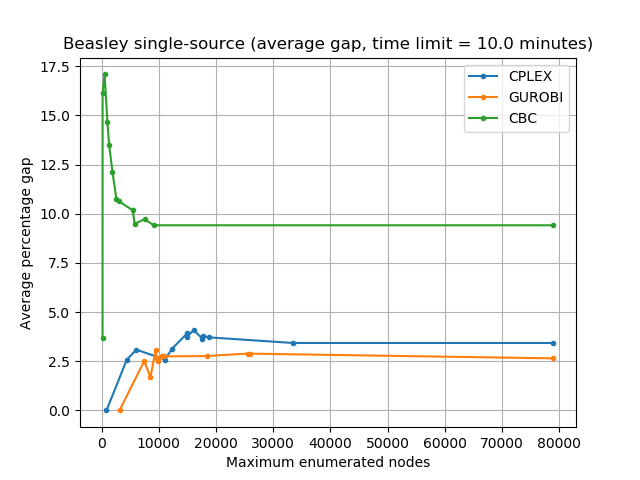
\includegraphics[width=0.49\textwidth]{res/Beasley SS large 600 - Average gap x Nodes.png}
				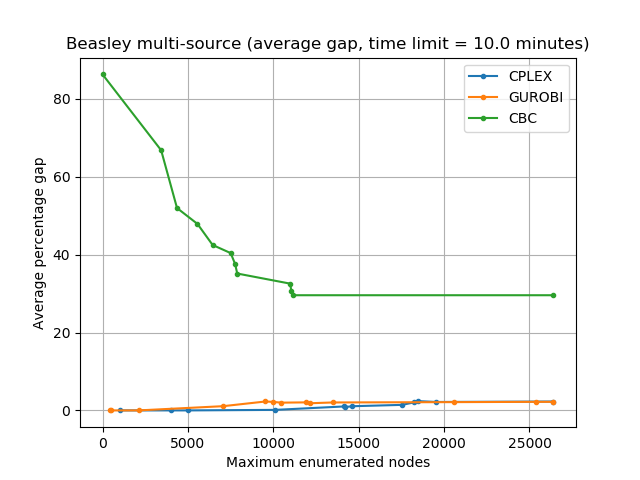
\includegraphics[width=0.49\textwidth]{res/Beasley MS large 600 - Average gap x Nodes.png}				
				\label{Gap:n:Beasley:600}
				
				\textbf{Fonte}: autoria própria.
			\end{center}
		\end{figure}
		
	\end{frame}
	
	
	\begin{frame}{Resultados: categoria 1 (2 minutos)} % Sobolev 120 SS Opt/n
		%\framesubtitle{}
		
		\begin{figure}[H]
			\begin{center}
				\caption{Instâncias médias resolvidas com otimalidade em até $x$ nós e 2 minutos SS-CFLP \cite{Sobolev}}
				
				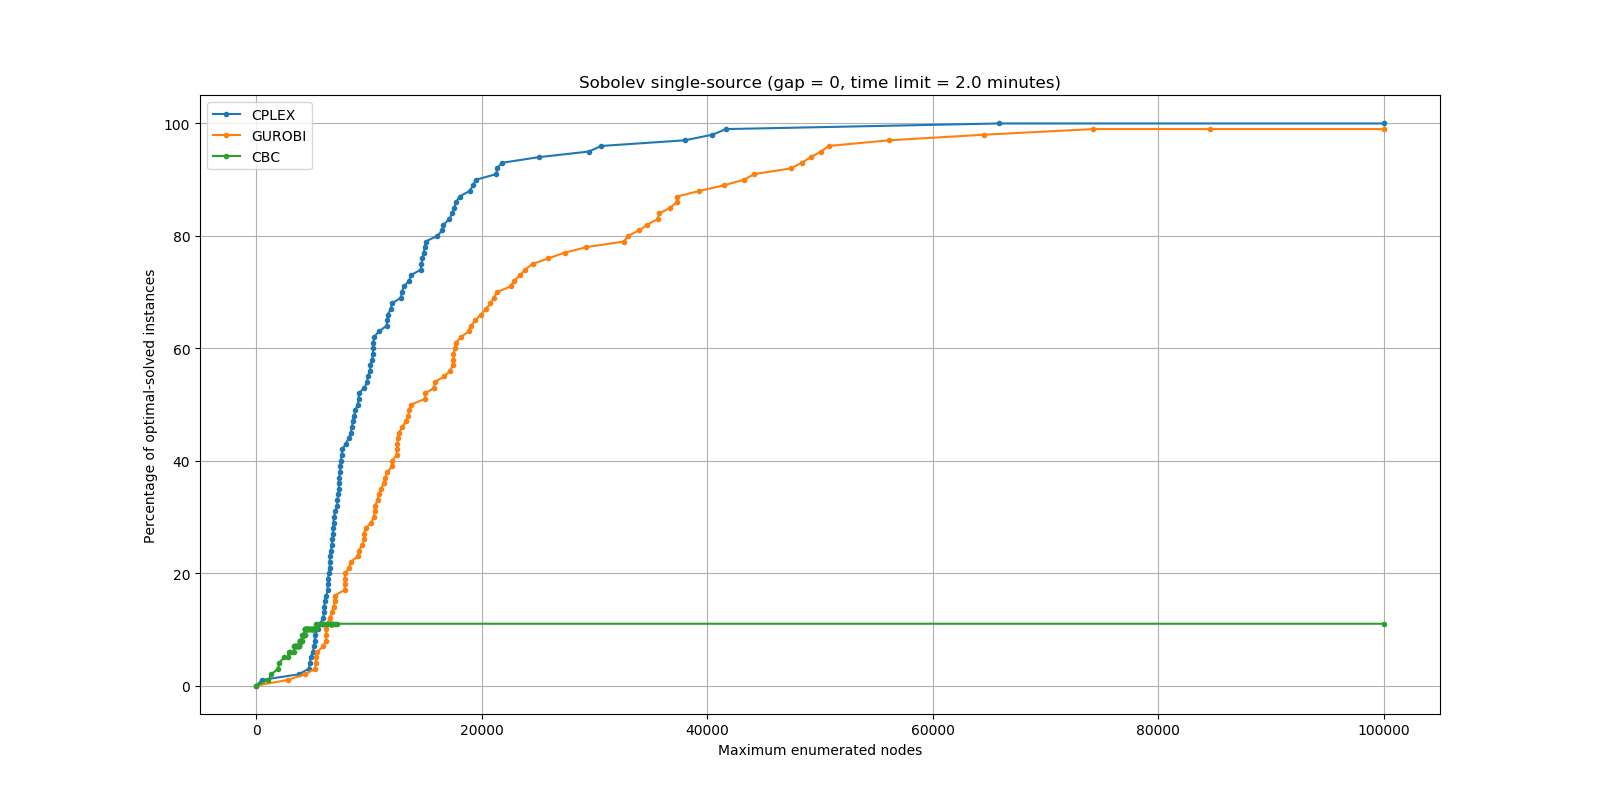
\includegraphics[height=0.6\textheight]{res/Sobolev SS 120 - Optimal x Nodes.png}
				\label{Opt:n:SS:Sobolev:120}
				
				\textbf{Fonte}: autoria própria.
			\end{center}
		\end{figure}
		
	\end{frame}

	\begin{frame}{Resultados: categoria 1 (5 minutos)} % Sobolev 300 SS Opt/n
		%\framesubtitle{}
		
		\begin{figure}[H]
			\begin{center}
				\caption{Instâncias médias resolvidas com otimalidade em até $x$ nós e 5 minutos SS-CFLP \cite{Sobolev}}
				
				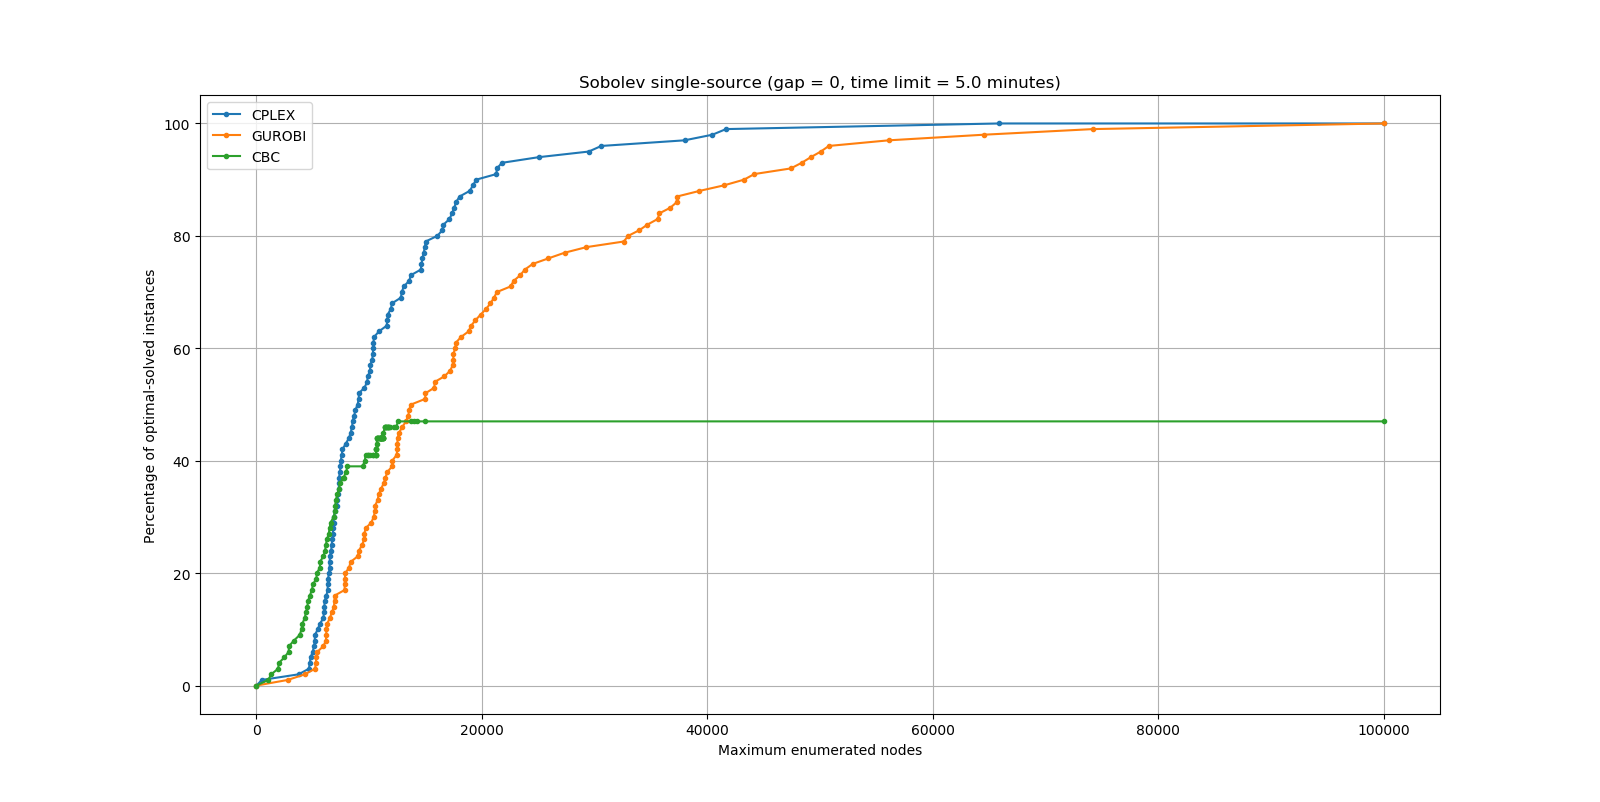
\includegraphics[height=0.6\textheight]{res/Sobolev SS 300 - Optimal x Nodes.png}
				\label{Opt:n:SS:Sobolev:300}
				
				\textbf{Fonte}: autoria própria.
			\end{center}
		\end{figure}
		
	\end{frame}
	
	\begin{frame}{Resultados: categoria 1 (10 minutos)} % Sobolev 600 SS Opt/n
		%\framesubtitle{}
		
		\begin{figure}[H]
			\begin{center}
				\caption{Instâncias médias resolvidas com otimalidade em até $x$ nós e 10 minutos SS-CFLP \cite{Sobolev}}
				
				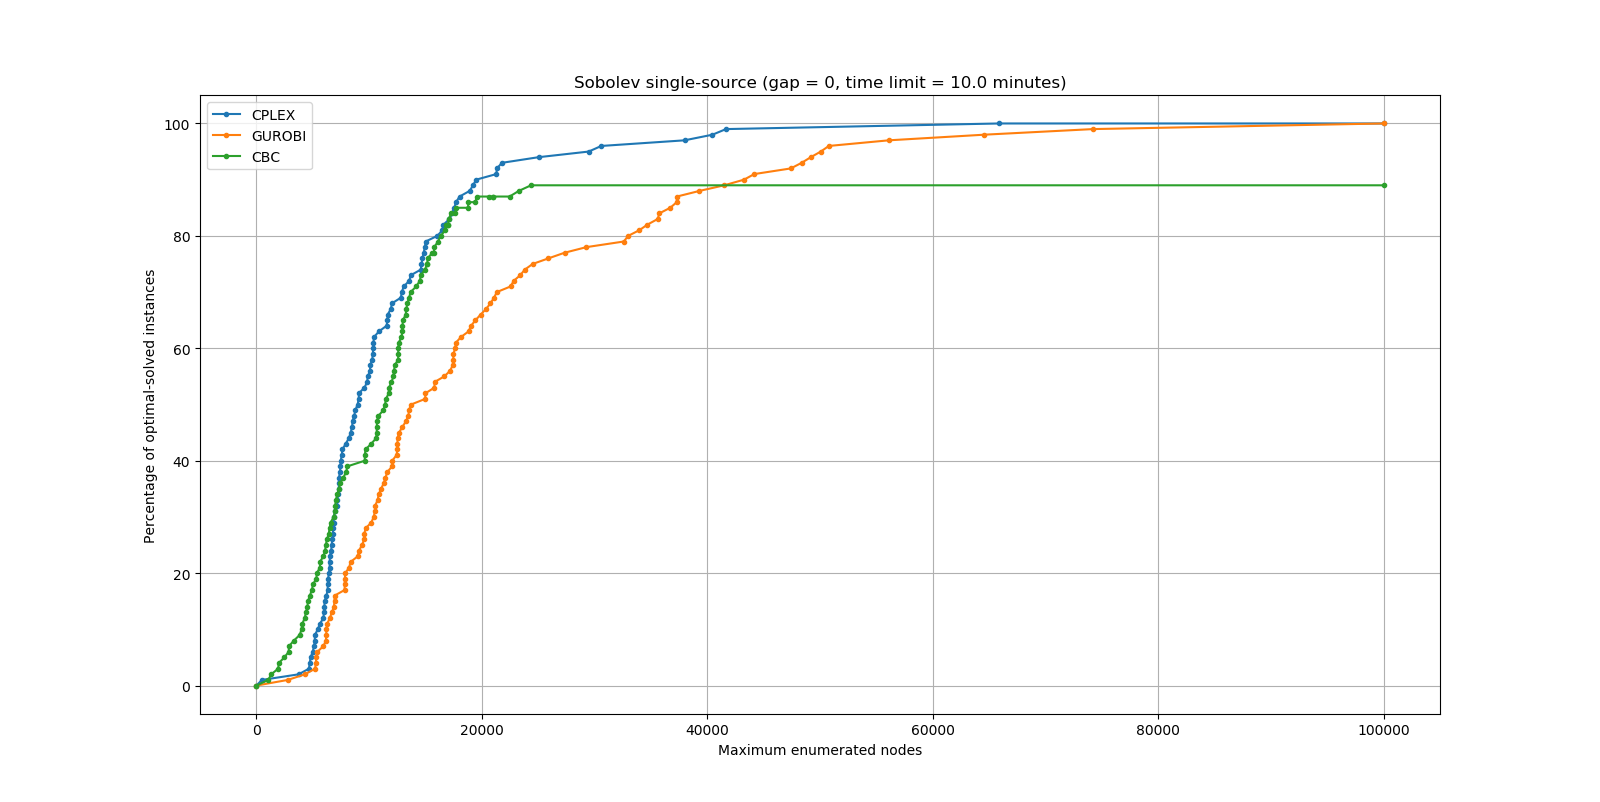
\includegraphics[height=0.6\textheight]{res/Sobolev SS 600 - Optimal x Nodes.png}
				\label{Opt:n:SS:Sobolev:600}
				
				\textbf{Fonte}: autoria própria.
			\end{center}
		\end{figure}
		
	\end{frame}
	
	\begin{frame}{Testes: categoria 3}
		
		
		Limite de tempo de 10, 30 e 60 minutos
		\\ \hfill \\
		Computador laptop Windows 10 (i7 64-bit RAM 16 GB)				
		\\ 2 núcleos físicos, 4 processadores lógicos
		
		%Utilizados os limites de tempo de 2, 5 e 10 minutos para todas as instâncias pequenas, médias e grandes dos MS e SS-CFLP \cite{Beasley,Sobolev} num c.
			
		%Para as instâncias do MS-CFLP-CI \cite{Maia} foram utilizados 10, 30 e 60 minutos num .
	\end{frame}

	\begin{frame}{Resultados: categoria 3 (múltiplas fontes com incompatibilidades de clientes)} % Maia MS CI Opt/T
		%\framesubtitle{}
		
		\begin{figure}[H]
			\begin{center}
				\caption{Instâncias muito grandes resolvidas com otimalidade pelo tempo limite MS-CFLP-CI \cite{Maia}}
				
				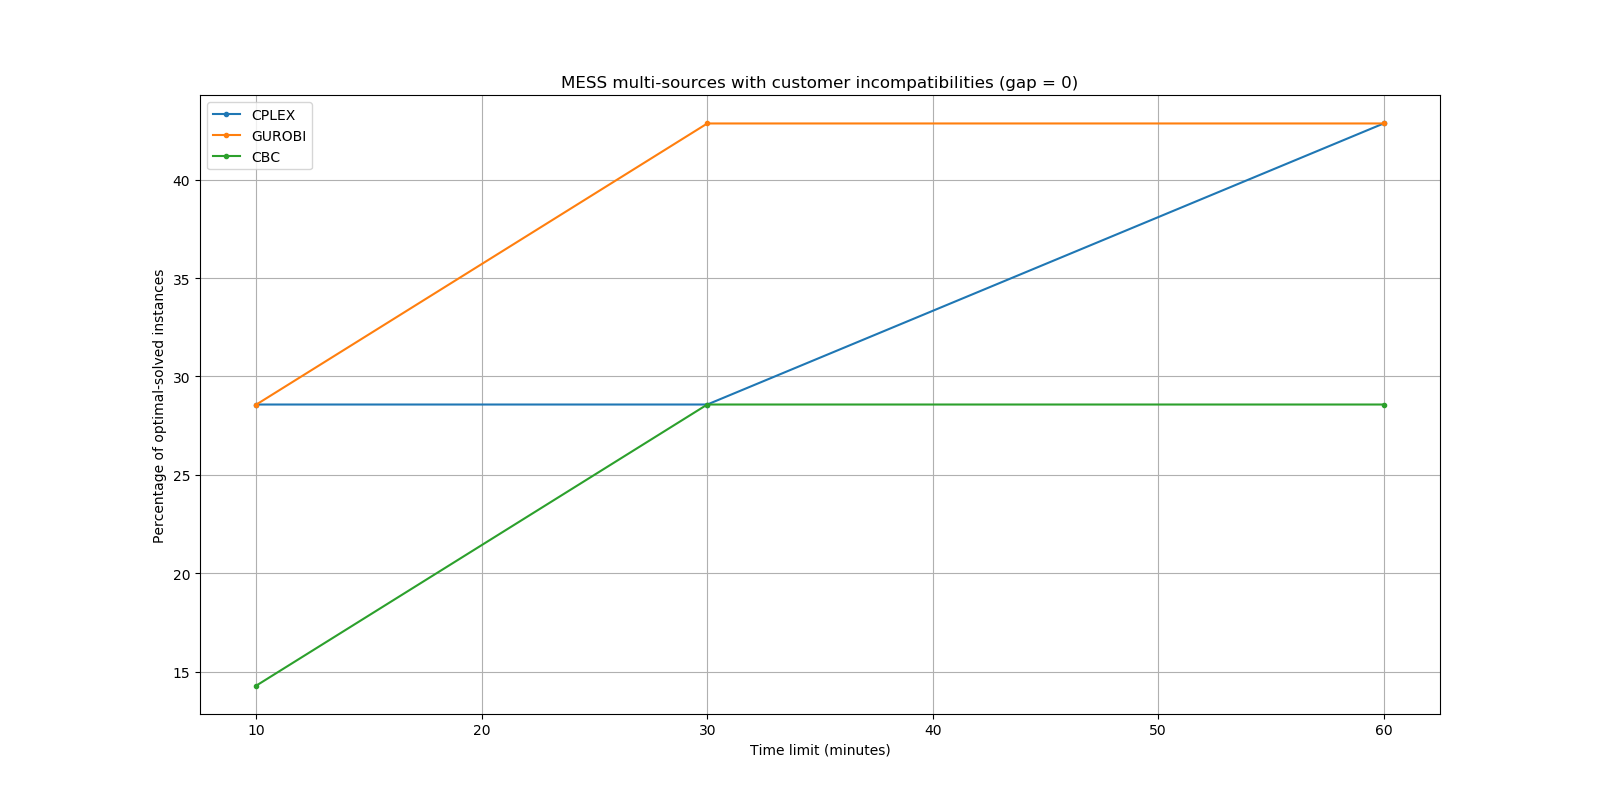
\includegraphics[height=0.6\textheight]{res/MESS MS CI - Optimal x Time.png}
				\label{Opt:T:MS:CI:Maia}
				
				\textbf{Fonte}: autoria própria.
			\end{center}
		\end{figure}
		
	\end{frame}

	\begin{frame}{Resultados com incompatibilidade de clientes} %  problemas do MS-CFLP-CI 
		\framesubtitle{Problemas com as instâncias muito grandes do MS-CFLP-CI} 
		
		Das 20 instâncias muito grandes \cite{Maia}, somente 6 foram possíveis de resolver.
		
		\begin{multicols}{2}
		
			\textbf{No desktop Ubuntu}:
			\begin{itemize}
				
				\item 
					\solver{CPLEX}: 
					3ª instância (244 kB)
					\\ esgotou a memória RAM em menos de 5 minutos  
				
				\item 	
					\solver{Cbc}: 
					4ª instância (449 kB)
					\\ falhou já no primeiro limite (10 minutos)
					
				\item	
					\solver{Gurobi}: 
					4ª instância
					\\ falhou no limite de 60 minutos
				
			\end{itemize}
		
			\hfill \\ \hfill \\
			\textbf{No laptop Windows}:				
			
			\begin{itemize}
				
				\item 	
					\solver{Cbc}: 
					4ª e 5ª instância (709 kB)
					\\ falhou no primeiro limite (10 minutos)
					\\ 6ª instância (983 kB) 
					\\ não funcionou para nenhum tempo limite
				
				\item 
					\solver{CPLEX}: 
					6ª instância
					\\ falhou no limite de 60 minutos  
				
				\item	
					\solver{Gurobi}: 
					7ª instância (1.85 MB)
					\\ em quase 48h, não havia terminado de ler o modelo 
				
			\end{itemize}
		 
		\end{multicols}
		
		
		
		
	\end{frame}	

	\begin{frame}{Considerações finais} % 
		%\framesubtitle{}
		
		%O \solver{CPLEX} teve mais soluções ótimas e menor gap médio em quase todos os casos, com exceção das instâncias grandes SS-CFLP \cite{Beasley}, em que o \solver{Gurobi} teve melhor desempenho nessas duas métricas. 
		%Porém, como um todo, não se diferenciaram significativamente nessas métricas para nenhum dos testes realizados.
		\textbf{Desempenho geral}: 
		\solver{CPLEX}, 
		seguido do \solver{Gurobi} 
		e \solver{Cbc}.  
		
		\hfill \\ \textbf{Uso do processamento}:
		o \solver{Cbc} não utilizou toda a capacidade de processamento disponível.

		\hfill
		\\
		Os resolvedores comerciais atingiram otimalidade para todas as 100 instâncias médias SS-CFLP (categoria 1), o \solver{Cbc} obteve os seguintes gaps médios:		
		\\	\textbf{Até 2 minutos}:	5.091518 \%
		\\	\textbf{Até 5 minutos}:	2.657762 \%
		\\	\textbf{Até 10 minutos}:	0.095106 \%
		
		\hfill \\ O problema MS-CFLP-CI é mais difícil de resolver e as instâncias da categoria 3 são muito grandes.   
		Outras técnicas de resolução precisam ser exploradas como, por exemplo, métodos de decomposição.
		
		
	\end{frame}
	
	
	\begin{frame}{Referências bibliográficas}
	%	\frametitle
		
		\bibliography{ref.bib}
		
		
	\end{frame}
	
	
	
	\begin{frame}{Agradecimentos}
		%\frametitle
		
		\quad \hfill			
				\href{https://www.uel.br/pos/pgmac/?content=PICME.htm}{\includegraphics[width=0.24\textwidth]{Logo_PICME_curto.png}}
			\hfill	
				\href{http://cnpq.br/}{\includegraphics[width=0.31\textwidth]{Logo_CNPq.png}}
		\hfill \quad	
	
	
	
	\end{frame}
	
	\begin{frame} % título final
		\maketitle
	\end{frame}


\end{document}
